% !TEX root = ../main.tex
% !TeX spellcheck = fr_FR

\chapter{Caractéristiques d'une passerelle pour \ac{LLN}}
\label{gw}

\epigraph{We build too many walls and not enough bridges.}{Isaac Newton}

\minitoc

Ce chapitre considère les différentes solutions techniques existantes pouvant être adoptées notamment à la passerelle pour déployer un \ac{LLN}.
Les choix techniques effectués dans cette thèse seront justifiés en prenant en compte les fonctionnalités souhaitées.

La section~\ref{gw:interop} couvre les contraintes d'interopérabilité au travers d'une présentation des différentes solutions d'accès sans-fil aux nœuds et détaille comment les connecter à un réseau IP classique en leur fournissant un adressage commun.

La section~\ref{gw:routing} couvre les contraintes liées au routage dans les \ac{LLN} et motive les choix faits dans cette thèse.

La section~\ref{gw:app_layer} aborde comment des fonctionnalités d'interfaces applicatives efficaces peuvent être déployées sur la passerelle afin d'améliorer la rapidité des requêtes et faciliter leur intégration avec des services déjà existants.

La section~\ref{gw:supervision} présente les fonctionnalités de supervision déployables sur la passerelle et comment elles peuvent être appliquées pour connaître l'état des nœuds.

La section~\ref{gw:conclusion} conclut ce chapitre, récapitule les choix techniques effectués et introduit les contributions relatives à la passerelle couvertes dans les chapitres suivants.

\section{Technologie sans-fil et adressage}
\label{gw:interop}

Comme expliqué dans le chapitre~\ref{intro}, les \ac{LLN}s mettent en jeu des nœuds hétérogènes avec des architectures matérielles très variées.
Les spécificités propres à chaque nœud doivent être masquées pour les administrateurs et fournisseurs de services afin qu'ils puissent se concentrer sur le développement de service à valeur ajoutée plutôt que sur les particularités de chaque nœud.
% Il n'est pas envisageable que chaque nœud adopte un langage universel (car il n'assurerait pas de compatibilité avec de nouvelles versions du langage, et le supporter sur les nœuds déjà déployés n'est pas forcément possible en pratique).
Dans cette thèse, on considère donc que cette opération est déportée sur une passerelle qui est plus adaptée en raison de sa position d'interface et des ressources supplémentaires dont elle dispose.

D'un point de vue matériel, une passerelle est un équipement réseau disposant d'au moins une interface connectée au \ac{LLN} et d'au moins une interface connectée à un réseau classique fonctionnant par exemple avec IP.
Cette passerelle dispose de plus de ressources qu'un nœud capteur et peut rester éveillée en permanence.
Elle peut être administrée via une interface graphique comme une interface web.

\subsection{Communication vers \ac{LLN}s}
\label{gw:low_layers}

Des solutions filaires comme le \ac{PoE} permettent de fournir alimentation électrique et connectivité aux capteurs.
Cependant, ces solutions filaires peuvent être très coûteuses et difficiles à déployer, notamment dans de grandes zones ouvertes et difficiles d'accès.

Les technologies sans-fil apportent une solution efficace et pratique de connectivité pour l'\ac{IoT} en utilisant pour leurs transmissions des bandes de fréquences \ac{ISM} qui présentent l'avantage d'être libre de droits et ne nécessitent donc pas de licence.
Les \ac{LLN}s s'appuient sur ces technologies sans-fil afin de simplifier les déploiements et réduire leurs coûts opérationnels.

Plusieurs solutions sont disponibles~\cite{wifiCritic} chacune d'elle offrant un compromis entre la bande passante, la portée et la consommation énergétique des équipements mis en jeu.
On peut distinguer deux grandes catégories de technologies sans-fil~: d'une part celle offrant un accès de longue portée (plusieurs kilomètres) et d'autre part celle offrant un accès de courte portée (moins d'un kilomètre).

\subsubsection{Accès longue portée}
\label{gw:long_range}

Les accès de type cellulaire permettent de fournir un accès Internet a un grand nombre d'appareils mobiles~\cite{kim2007value}.
Cependant ils ne sont pas adaptés au cas des \ac{LLN}s, d'une part en raison du prix de fabrication des composants radios dont ils ont besoin, du coût de l'accès (licence, abonnement auprès d'un opérateur) et d'autre part par la consommation énergétique qu'ils induisent.
Ainsi des technologies plus adaptées aux \ac{LLN}s sont requises pour offrir des accès longues portées.

Les technologies dites \ac{LPWAN} permettent de transmettre un volume de trafic faible~\footnote{Environ 200 octets (typique) à 5000 octets (maximum) émis par jour avec une charge applicative utile de l'ordre de 12 octets} sur des distances longues~\footnote{5 à 40 kilomètres en champ libre} à un faible débit~\footnote{Débit de 10 à 1 kbit/s en fonction de la technologie radio}~\cite{xiong2015low}.

Ces technologies offrent un jeu de compromis clair~: peu de débit, une grande portée, une bonne pénétration~\footnote{Important pour des objets situés dans des caves comme des compteurs électriques.}, un coût de composant radio faible~\footnote{Moins de 2 dollars} et qui consomme très peu d'énergie.

Cependant, ces technologies présentent plusieurs limitations.
Les stations de base lorsqu'elles émettent utilisent une puissance supérieure à celle autorisée pour les usages privés (four à micro-ondes, Wi-Fi, etc.) sur les bandes \ac{ISM}~\cite{rec200170}.
Dans ces conditions, les autorités régulatrices de l'utilisation des bandes \ac{ISM} obligent les stations de base à ne pas transmettre au plus que 1 \% de leur temps~\cite{vangelista2015long}.

De plus, les bandes de fréquences \ac{ISM} utilisées étant étroites, les liens descendant et montant sont très proches.
Ainsi, les stations ne peuvent pas actuellement transmettre vers les objets tout en écoutant avec le même niveau de sensibilité les autres nœuds de leur cellule.
Donc dans le cas où il faut fournir un service de lien descendant (par exemple pour acquitter un paquet, mettre à jour un objet, ou déclencher des actions) l'utilisation de ces technologies doit se faire dans un contexte où le nombre de stations est surdimensionné afin d'offrir une bonne qualité de service.
Par conséquent, si le nombre d'objets devient grand il devient nécessaire de densifier le nombre de stations de base pour fournir un canal de communication satisfaisant des stations vers les objets ce qui augmente les coûts de déploiements.

La 5G, annoncée pour l'horizon 2020, entend regrouper et intégrer ce type de technologies longue portée pour une utilisation plus efficace des bandes de fréquences qui seront alors disponibles.

En pratique, les \ac{LPWAN}s sont orientés vers des applications où les objets publient des messages sans confirmation de leur réception (par exemple: un relevé de compteur effectué quotidiennement) et reçoivent encore moins de trafic de la part des stations de base.
Ces applications principales concernent les relevés d'informations d'équipements et de télémétries journalières.

\subsubsection{Accès courte portée}
\label{gw:short_range}

Les technologies sans-fil de courte portée offrent une alternative permettant d'avoir une bande passante et un débit plus important tout en offrant une meilleure fiabilité des transmissions.
Cependant l'utilisation de ces technologies impose un nouveau jeu de compromis.

Les nœuds peuvent être loin de la passerelle qui les connecte au reste du réseau, ainsi l'utilisation de topologies de réseau maillé est nécessaire afin d'offrir une connectivité à des nœuds étant loin de la passerelle.

Les bandes \ac{ISM} sont très chargées par de multiples appareils comme les micro-ondes ou bien d'autres appareils utilisant le Wi-Fi.
Ainsi il est nécessaire pour des nœuds d'un \ac{LLN} de disposer de mécanismes pour éviter d'avoir leurs signaux écrasés par d'autres stations émettant avec des puissances plus fortes.

D'autre part, les signaux peuvent suivre plusieurs chemins entre deux nœuds en raison des réflexions causées par l’environnement.
Ainsi un même signal peut arriver avec des amplitudes différentes et des phases différentes pouvant causer des interférences et des pertes (appelé en anglais ``multipath-fading'').
Ces conditions sont très instables et dépendent de l'utilisation d'une fréquence donnée, dans un environnement donné, à un temps donné.

Les technologies sans-fils de portée courte sont nombreuses, et seules les plus représentatives seront abordées dans les paragraphes suivants.

\paragraph{Wi-Fi}

Le Wi-Fi facilite l'utilisation d'Internet sur un grand nombre de périphériques mobiles en proposant un accès natif à un réseau IP avec des débits importants~\cite{lee2010mobile}.

Cependant, une puce Wi-Fi est coûteuse, d'une part par sa puce radio qui est coûteuse à fabriquer et d'autre part par sa consommation d'énergie~\cite{wifiCritic}.
En outre, son débit est très souvent surdimensionné par rapport aux besoins des nœuds.

De nouvelles technologies sans-fil ont donc ont été conçues afin de transporter des messages à des débits plus modeste tout en consommant moins d'énergie et en restant sur les bandes \ac{ISM}.

\paragraph{Z-wave}

Z-wave permet de connecter des objets dans une topologie maillée principalement dans le secteur domotique.
Cette technologie permet d'avoir des communications fiables, avec une faible latence et un débit maximal de 100 kbit/s.

Son attrait se trouve dans sa large diffusion dans le secteur de la domotique avec une large gamme de produits compatibles entre eux~\cite{zwaveCritic}.

Cependant Z-wave ne permettent pas de passer simplement à l'échelle~\footnote{Limitation à 4 routeurs intermédiaires pour un réseau maillé, pas plus de 232 nœuds par réseau.} sur des scénarios avec un grand nombre de nœuds comme un bâtiment entier, une ville ou un centre commercial qui sont des cas d'utilisation importants des \ac{LLN}s~\cite{zwaveCritic}.

\paragraph{\ac{BLE}}

\ac{BLE} est une spécification complète de l'ensemble de la pile protocolaire des couches basses jusqu'à l'applicatif visant les \ac{PAN} et qui permet de connecter des objets dans une topologie en étoile sur des portées d'une dizaine de mètres.

Typiquement utilisée pour des appareils personnels (montre et bracelet connectés, accessoires de sport), cette spécification dispose de beaucoup d'atouts: un débit important (1Mo/s) permettant de passer peu de temps à émettre, des entêtes réduits, une grande efficacité spectrale et un schéma de saut de fréquence pour éviter les canaux chargés typiques des bandes \ac{ISM}.

Cependant les portées de transmissions sont encore trop limitées et le support des réseaux maillés avec cette technologie n'est pas encore standardisé~\cite{bleCritic}.

\paragraph{\ieee{}}

\ieee{} permet de connecter des objets disposant de ressources limitées entre eux par une topologie étoilée, maillée ou arborescente sur des portées de 10 à 50 mètres avec des débits de 250kbit/s.
\ieee{} est utilisée par plusieurs normes~\footnote{Zigbee~\cite{alliance2006zigbee, zigbeeCritic}, Wireless HART~\cite{lennvall2008comparison}, EnOcean~\cite{ploennigs2010performance}, \ac{6LoWPAN}~\cite{shelby20116lowpan} et plus récemment Thread~\cite{threadCritic}} ainsi ces normes permettent de disposer d'une large littérature sur ses performances et son fonctionnement.
% \ieee{} permet des communications bidirectionnelles plus flexibles avec des débits plus élevés contrairement à ce que propose les accès~\ac{LPWAN} ce qui est pertinent dans des cas où des besoins de bande passante plus élevés sont souhaitables pour envoyer une photo de surveillance par exemple.
En outre, sa consommation énergétique est faible de même que le coût moyen de ses composants radios physiques~\cite{vilajosana2015openmote}.

De plus, des techniques basées sur des sauts de fréquences sont intégrées dans les spécifications les plus récentes de \ieee{} et permettent d'augmenter sa fiabilité et de mitiger les problèmes dus au multi-path fading~\cite{6tisch}.

\paragraph{Conclusion intermédiaire}

\begin{table*}[t]
\centering
\begin{tabular}{|l|c|c|c|c|c|}
\hline
Protocole & Saut de fréquence & Débit & Topologie & Pile complète \\
\hline
LPWAN & Non & 100 à 1200 bps & Étoile & Non \\
\hline
Wi-Fi & Non & 248 Mbps & Étoile, Maillé & Non \\
\hline
Z-wave & Non & 9.6, 40, 100 kbps & Étoile, Maillé &  Oui \\
\hline
\ac{BLE} & Oui & 250 kbps & Étoile & Oui \\
\hline
\ieee{} & Possible & 250 kbps & Étoile, Maillé & Non \\
\hline
\end{tabular}
\caption{Récapitulatif des protocoles sans-fil}

\label{gw:table:protocol_recap}
\end{table*}

Le tableau~\ref{gw:table:protocol_recap} offre un récapitulatif des technologies sans-fil considérée.
Après analyse des différentes solutions possibles, \ieee{} est le protocole qui apparaît comme le plus adapté pour construire des réseaux maillés permettant de pallier efficacement à la faible portée des nœuds en augmentant la couverture et cela sans limites de nœuds.

Pour cette raison, le travail effectué dans cette thèse s'appuie exclusivement sur \ieee{}.

\subsection{Plan d'adressages dans un \ac{LLN}}
\label{gw:ip}

D'un point de vue fonctionnel, dans un réseau maillé, on distingue les hôtes simples représentés par un H sur la Figure~\ref{gw:fig:arch_6lowpan} et les routeurs représentés par un R.
Les hôtes envoient et reçoivent des messages, mais n'en transfèrent pas pour le compte d'autres nœuds.
Les routeurs font suivre des paquets entre leur origine et leur destination.
Il est à noter qu'un routeur peut également recevoir et envoyer des messages et assurer les deux fonctions (routeur et hôte).

Au vu de cette répartition des rôles dans un \ac{LLN}, il y a essentiellement trois types d'architectures possibles représentées sur la Figure~\ref{gw:fig:arch_6lowpan}.

La plus simple consiste en un \ac{LLN} connecté de manière ad hoc.
Les nœuds hôtes envoient des informations que les nœuds routeurs relaient vers leurs destinations.
Ce type de déploiement est par exemple utilisé dans des déploiements sur des terrains sans connectivité avec un autre réseau~\cite{werner2006deploying}.

Le second type de déploiement utilise une passerelle pour assurer le rôle de routeur de bordure entre le \ac{LLN} et un réseau local.
Ce type de déploiement peut par exemple se retrouver dans un scénario domotique dans lequel tous les équipements communiquent vers la même passerelle.

Enfin un dernier type de déploiement étend le scénario du routeur de bordure pour prendre en charge le cas où des nœuds peuvent avoir plusieurs passerelles vers un réseau commun.
Ce type de déploiement peut être pertinent dans le cas où les nœuds capteurs sont mobiles et doivent pouvoir changer de passerelles tout en restant connectés au réseau et en ne changeant pas leur adresse.

Toutes ces architectures requièrent un adressage de chaque nœud afin de pouvoir garantir des communications en unicast qui sont importantes pour économiser de l'énergie et du débit par rapport à des communications broadcast.

\ieee{} fournit un plan d'adressage pour chaque nœud du \ac{LLN}, cependant ces adresses ne sont pas utilisables à l'extérieur de ce réseau.
Ainsi un utilisateur voulant mettre l'ensemble de ses équipements (capteurs, machines classiques) sur le même plan d'adressage afin de simplifier sa gestion ne peut le faire avec cette solution.
Une passerelle est donc requise pour faire une éventuelle traduction entre l'adressage du réseau standard et les \ac{LLN}s.

Afin de limiter la consommation d'énergie, la passerelle doit pouvoir contacter les nœuds d'un \ac{LLN} individuellement, car parler systématiquement à l'ensemble des nœuds serait coûteux pour un grand réseau et ne permettrait aucun mécanisme d'authentification.

Ainsi la passerelle doit disposer d'un plan d'adressage qui permet d'atteindre chaque nœud d'un \ac{LLN}.

\begin{figure}[ht]
  \centering
  \begin{tikzpicture}

  % définition des styles
  \tikzstyle{visible}=[draw, fill=blue!50]
  \tikzstyle{hidden}=[ draw, fill=gray!20]
  \tikzstyle{router}=[circle, draw, fill=orange!50,text=black]
  \tikzstyle{child}=[circle, draw, fill=yellow!50,text=black]
  \tikzstyle{root}=[circle, draw, fill=red!50,text=black]

  % Ad-hoc
  \node[router] (1) at (-4, 0) {R};
  \node[router] (2) at (-5, 1) {R};
  \node[child] (3) at (-5, -1) {H};
  \node[child] (4) at (-6, 2) {H};
  \node[child] (5) at (-6, 0) {H};
  \node [fit=(1) (2) (3) (4) (5), rounded corners, draw=black!50] (lln) {};
  \node [below=.3 cm of lln] {Ad-hoc};

  \path

  % Réseau contraint
  (1) edge[<->] (2)
  (1) edge[<->] (3)
  (2) edge[<->] (4)
  (2) edge[<->] (5)
  ;

  % Simple
  \node[router] (11) at (-1, 0) {R};
  \node[router] (21) at (-2, 1) {R};
  \node[child] (31) at (-2, -1) {H};
  \node[child] (41) at (-3, 2) {H};
  \node[child] (51) at (-3, 0) {H};
  \node[visible, above=of 21] (simplelbr) {LBR};
  \node [fit=(11) (21) (31) (41) (51) (simplelbr), rounded corners, draw=black!50] (simple) {};
  \node [below=.3 cm of simple] {Simple};

  \path

  % Réseau contraint
  (simplelbr) edge[<->] (21)
  (11) edge[<->] (21)
  (11) edge[<->] (31)
  (21) edge[<->] (41)
  (21) edge[<->] (51)
  ;

  % Etendu
  \node[router] (111) at (2, 0) {R};
  \node[router] (211) at (1, 1) {R};
  \node[router] (711) at (3, 1) {R};
  \node[child] (311) at (1, -1) {H};
  \node[child] (611) at (3, -1) {H};
  \node[child] (411) at (0, 2) {H};
  \node[child] (511) at (0, 0) {H};
  \node[visible, above=of 211] (lbr1) {LBR};
  \node[visible, right=1.2cm of lbr1] (lbr2) {LBR};
  \node [fit=(111) (211) (311) (411) (511) (611) (lbr1) (lbr2), rounded corners, draw=black!50] (etendu) {};
  \node [below=.3 cm of etendu] {Étendu};

  \path

  (lbr1) edge[<->] (lbr2)
  (211) edge[<->] (lbr1)
  (211) edge[<->] (lbr2)
  (711) edge[<->] (lbr1)
  (711) edge[<->] (lbr2)
  (111) edge[<->] (211)
  (111) edge[<->] (311)
  (211) edge[<->] (411)
  (211) edge[<->] (511)
  (611) edge[<->] (711)
  (211) edge[<->] (711)
  (111) edge[<->] (711)
  ;

  \end{tikzpicture}

  \caption{Architecture réseau des \ac{LLN}s}
  \label{gw:fig:arch_6lowpan}  
\end{figure}

\subsubsection{IPv4}
\label{gw:ipv4}

IP étant le protocole réseau le plus utilisé aujourd’hui il est un candidat naturel pour fournir un adressage sur un \ac{LLN} qui soit interopérable avec un réseau existant.
Ainsi une solution consisterait à affecter une adresse IPv4 à chaque nœud.

Toutefois, IPv4 n'est pas pleinement satisfaisant principalement pour deux raisons.
D'une part la pénurie d'adresses IPv4~\cite{deering1998internet} ne permet pas d'assigner une IP publique à chaque nœud ce qui est dommageable dans le cas où des scénarios de connexions directs sont requis.
Une solution consisterait à utiliser des \ac{NAT}s~\footnote{Mécanisme permettant de disposer de plusieurs adresses privées derrière une seule adresse publique.} afin de pallier au manque d'adresses publiques allouées.
Cependant, des \ac{NAT}s requièrent de reconstruire des paquets et ce traitement dégraderait les performances en plus d'être complexe et d'invalider la connexion de bout en bout directe.

D'autre part, les en-têtes IPv4 sont relativement grands, ce qui signifie plus d'informations à transmettre et donc plus d'énergie à consommer pour transmettre un message.
Ceci pourrait être clairement amélioré puisqu'un en-tête IPv4 véhicule des informations qui ne sont pas pertinentes pour un \ac{LLN} (type de service, padding, etc.)~\cite{shelby20116lowpan}.

\subsubsection{IPv6}
\label{gw:ipv6}

Une solution alternative consiste à utiliser IPv6 afin de disposer d'un vaste espace d'adressage rendant l'utilisation d'un \ac{NAT} superflue et qui permettrait de généraliser les connexions de bout en bout sans intermédiaire.
Cependant l'utilisation d'IPv6 comporte des inconvénients dans le cas des \ac{LLN}s.
L'entête de taille fixe d'IPv6 (40 octets) est plus large que celle d'IPv4 (20 octets), d'autre part, IPv6 définit un \ac{MTU} \emph{minimal} de 1280 octets afin d'éviter les problèmes de fragmentation et de recomposition de paquets.
Or \ieee{} ne peut fournir au maximum qu'une trame de 127 octets, ainsi les paquets IPv6 venant de \ieee{} serait rejetés par un routeur IPv6 implémentant ces recommandations de \ac{MTU} minimal.

Actuellement, IPv4 est encore largement déployé et donc les adressages IPv4 et IPv6 vont cohabiter plusieurs années~\cite{colitti2010evaluating}.
Si un \ac{LLN} utilise IPv6 pour son adressage et qu'il doit pouvoir recevoir des instructions envoyées depuis un réseau standard fonctionnant en IPv4 alors la passerelle doit assurer une conversion IPv4/IPv6 qui peut être effectuée par un mécanisme de traduction (teredo, 6to4, isatap, etc.)~\cite{conta1998generic}.

Pour transmettre des messages, il est nécessaire d'indiquer un protocole de transport pour les acheminer.
Le protocole de trafic le plus compact en terme d'en-têtes considéré dans le cadre des \ac{LLN}s est \ac{UDP}.
En effet, comparé à \ac{TCP}, il requiert moins d'espace dans l'en-tête du paquet (diminuant ainsi son coût en énergie) et n'utilise pas d'acquittements (limitant ainsi le nombre de messages et donc la consommation d'énergie).
Dans le cas où les messages doivent être acquittés, ils peuvent l'être avec un mécanisme ad hoc situé au niveau de la couche applicative.

\begin{figure}[ht]
	\centering
	% \begin{bytefield}[bitwidth=.3em]{127}
	\begin{bytefield}[bitwidth=.007\linewidth]{127}
		\bitheader[lsb=0]{23,23+21,23+21+40,23+21+40+8, 127} \\
		\colorbitbox{cyan}{23}{802.15.4}
		\colorbitbox{cyan}{21}{AES-CCM}
		\colorbitbox{Fuchsia}{40}{IPv6}
		\colorbitbox{orange}{8}{UDP}
		\colorbitbox{ForestGreen}{33}{{\footnotesize  DATA (33 octets)}}
		\colorbitbox{Salmon}{2}{\rotatebox{90}{\scriptsize FSC}}\\
		\colorbitbox{cyan}{23}{802.15.4}
		\colorbitbox{cyan}{21}{AES-CCM}
		\colorbitbox{Fuchsia}{40}{IPv6}
		\colorbitbox{LimeGreen}{20}{TCP}
		\colorbitbox{ForestGreen}{21}{{\footnotesize  DATA (21 octets)}}
		\colorbitbox{Salmon}{2}{\rotatebox{90}{\scriptsize FSC}}
		\end{bytefield}
	\caption{Trame 802.15.4 sur IPv6 (sans compression d'en-tête)}
	\label{gw:fig:802154}
\end{figure}

Une application directe de cette configuration est représentée sur la Figure~\ref{gw:fig:802154} qui représente une trame \ieee{} de donnée (``Data frame'' en anglais).
En \ieee{}, la taille maximale de données fournie par la couche physique (\ac{PLSDU}) est de 127 octets.
Utiliser IPv6 sans compression sur cette trame de données de 127 octets impliquerait de laisser seulement 33 octets utilisables pour des messages applicatifs puisque 25 sont pris par \ieee{}~\footnote{L'entête de sécurité représenté par AES-CCM sur la Figure~\ref{gw:fig:802154} est optionnel et peut consommer jusqu'à 21 octets}, 40 par IPv6 et 8 par \ac{UDP}; soit une efficacité de 26\%.
\ac{TCP} offre un rendement encore moins bon, car son entête prends plus de place que celle d'\ac{UDP}.
Afin d'améliorer ce rendement, il est nécessaire de procéder à une compression permettant d'empiler et d'abréger les informations contenues dans l'en-tête IPv6.
C'est ce que propose \ac{6LoWPAN}.

\subsubsection{6LoWPAN}
\label{gw:6lowpan}

\ac{6LoWPAN}~\cite{rfc4919} est une couche d'adaptation d'IPv6 à \ieee{} qui permet d'augmenter le rendement des trames.

\ac{6LoWPAN} définit entre autres, un format de trame pour la transmission des paquets, une méthode pour définir les adresses en lien local et des configurations d'adresses automatiques, la compression des entêtes et le processus de transfert de trames dans les réseaux maillés~\cite{rfc4944}.

\begin{figure}[ht]
	\centering
	% \begin{bytefield}[bitwidth=.3em]{127}
	\begin{bytefield}[bitwidth=.007\linewidth]{127}
		\bitheader[lsb=0]{23,44,44+7,44+7+4, 127} \\
		\colorbitbox{cyan}{23}{802.15.4}
		\colorbitbox{cyan}{21}{AES-CCM}
		\colorbitbox{Fuchsia}{7}{\rotatebox{90}{\scriptsize IPv6}}
		\colorbitbox{orange}{4}{\rotatebox{90}{\scriptsize UDP}}
		\colorbitbox{ForestGreen}{70}{DATA (70 octets)}
		\colorbitbox{Salmon}{2}{\rotatebox{90}{\scriptsize FSC}}\\
		\colorbitbox{cyan}{23}{802.15.4}
		\colorbitbox{cyan}{21}{AES-CCM}
		\colorbitbox{red}{5}{\rotatebox{90}{\scriptsize Frag}}
		\colorbitbox{Fuchsia}{7}{\rotatebox{90}{\scriptsize IPv6}}
		\colorbitbox{orange}{4}{\rotatebox{90}{\scriptsize UDP}}
		\colorbitbox{ForestGreen}{65}{DATA (65 octets)}
		\colorbitbox{Salmon}{2}{\rotatebox{90}{\scriptsize FSC}}
		\end{bytefield}
	\caption{Trame 802.15.4 avec entête de fragmentation et Entête IPv6 ``Header Compression''}
	\label{gw:fig:headers_6lowpan}
\end{figure}


Comme montré sur la Figure~\ref{gw:fig:headers_6lowpan}, la compression ne se fait pas au niveau du paquet tout entier car en cas de fragmentation et de perte d'un paquet il serait impossible de reconstituer le paquet original.
La compression se passe au niveau de l'entête IPv6 et de l'entête \ac{UDP} par deux mécanismes de compression~\cite{rfc4944}.

Afin de ne pas utiliser de processus complexes nécessitant de maintenir des états, les compressions sont sans états ou dépendent d'un contexte global à l'ensemble du \ac{LLN}~\cite{shelby20116lowpan}.
\ac{6LoWPAN} effectue une compression en retirant entre autres le préfixe IPv6 qui est le même au sein du réseau et en compressant les \ac{IID} qui sont basées sur l'adresse \ac{MAC} et déjà présentes dans les en-têtes \ieee{}.

Ainsi, \ac{6LoWPAN} permet de disposer de la compatibilité avec les réseaux IPv6 tout en disposant d'en-têtes compressés pour permettre de transmettre des messages applicatifs plus larges pouvant tenir dans la trame entière sans nécessiter de fragmentation.

\section{Routage}
\label{gw:routing}

Lorsqu'un \ac{LLN} utilise un réseau maillé pour communiquer (notamment en raison de la faible portée de transmission des nœuds), il est nécessaire de disposer d'un protocole de routage afin que les nœuds routeurs en charge de router les paquets puisse le faire.
Cependant les contraintes propres aux \ac{LLN}s se distinguent de celles des cas classiques de routage disponibles pour les réseaux usuels.

\subsection{Contraintes du routage dans les \ac{LLN}s}

L'objectif d'un protocole de routage pour \ac{LLN} est entre autres de minimiser la consommation d'énergie et de supporter les cycles de veille des nœuds en utilisant aussi peu de bande passante que possible.

\subsubsection{Faible empreinte sur les ressources d'un nœud}

Les routeurs utilisés dans les \ac{LLN}s sont généralement des nœuds capteurs eux-mêmes afin de simplifier les déploiements.
Ainsi, ces nœuds ne disposent généralement que d'une même interface radio pour traiter les paquets qu'ils doivent router pour le compte d'autres nœuds et leurs propres paquets.

De plus, les \ac{LLN}s mettent en jeu des nœuds fortement contraints ainsi un protocole de routage adapté doit induire aussi peu de signalisation que possible et doit nécessiter un faible espace mémoire.

En outre, le protocole de routage doit supporter les conditions imposées par les économies d'énergies (cycles de veille, bande passante limitée, \ldots).

\subsubsection{Détection des boucles}

Chaque équipement maintient dans sa table de routage quel voisin traverser pour joindre une destination.
Le protocole de routage doit maintenir ces routes qui doivent refléter la topologie courante du réseau, y compris si celle-ci est modifiée.
Dans ce genre de situation, les messages de routage permettent aux différents équipements de corriger leur table de routage.
Une telle correction, appelée convergence, peut prendre quelques (milli)secondes.
Cependant, rien ne garantit l'ordre dans lequel chaque routeur corrigera sa table de commutation, ni même que toutes les destinations seront joignables pendant que le réseau converge de nouveau.
Il arrive parfois que les paquets soient propagés de nouveau de manière incohérente et que des paquets soient propagés le long d'un cycle arbitraire sans jamais atteindre leur destination. 
On parle alors de boucle de routage.

Dans un réseau classique, une boucle de routage se traduit généralement par une saturation des interfaces mises en jeu dans la boucle (puisque les paquets s'accumulent dans la boucle), ce qui induit de la gigue sur les autres paquets amenés à traverser ces interfaces.
Le \ac{TTL} permet d'éviter qu'un paquet soit indéfiniment repropagé et donc limite ce phénomène.
Toutefois, un paquet dont le \ac{TTL} expire est jeté et est perdu, ce qui force sa source à le retransmettre (sous réserve qu'elle le détecte).

Dans un réseau \ac{LLN} une boucle de routage est encore plus négative.
D'une part l'utilisation d'\ac{UDP} au lieu de \ac{TCP} fait qu'une perte sera généralement définitive.
De plus, tout paquet capturé dans une boucle de routage engendre une perte sèche d'énergie, puisque la plupart du temps le paquet ne sera pas acheminé jusqu'à sa destination.

Pour toutes ces raisons, la détection d'une boucle de routage et son élimination est critique.

\subsubsection{Routage optimisé pour les types de trafic typiques des \ac{LLN}s}

Les protocoles de routages classiques comme \ac{OSPF}~\cite{rfc5340} ou \ac{BGP}~\cite{rfc4271} qui sont utilisés dans les réseaux classiques sont agnostiques concernant la direction et l'intensité du trafic émis.
Cependant, les \ac{LLN}s sont des ``stub networks'', ils disposent de leur réseau, mais ne font pas transiter de paquets pour d'autres réseaux: un nœud ne fera du routage que pour des nœuds appartenant au même réseau.
D'autre part, dans un \ac{LLN} les profils de trafic observés peuvent être répartis entre trois types de trafic.

\paragraph{\ac{MP2P}}

La mission essentielle des nœuds capteurs consiste à envoyer des relevés vers une racine, on parle alors de trafic remontant ou de \ac{MP2P}.
Ainsi la passerelle a un rôle prépondérant pour un protocole de routage puisqu'elle offre un  point de sortie pour chaque nœud qui veut envoyer des messages vers l'extérieur.
Donc, un protocole de routage idéal pour les \ac{LLN}s doit être optimisé pour ce type de trafic où les paquets en provenance des nœuds remontent vers une passerelle.

\paragraph{\ac{P2MP}}

Les nœuds capteurs peuvent aussi recevoir des paquets en unicast de la part de la passerelle on parle alors de trafic descendant ou \ac{P2MP}.
Ce type de trafic est représentatif de l'envoi d'une requête ciblée ou bien du déploiement d'une mise à jour sur un nœud capteur donné.

\paragraph{\ac{P2P}}

Les cas de trafic \ac{P2P} doivent être supportés, car ils sont possibles par exemple pour faire une découverte de ressources locales ou effectuer une action, mais ces cas sont minoritaires et le protocole de routage idéal doit concentrer ses optimisations sur les deux premiers types de trafic.

\subsection{Taxonomie des protocoles de routage}

Le routage dans les \ac{LLN}s a été étudié en profondeur pour le groupe de travail \ac{ROLL} de l'\ac{IETF}~\cite{draft-ietf-roll-protocols-survey-07}.
Leurs travaux ont permis d'aboutir à la conclusion qu'aucun protocole de routage disponible alors (2009) ne convenait sans modifications aux spécificités des \ac{LLN}s et qu'il était donc nécessaire d'en construire un.

Une brève description des principaux types de routage et de leur compatibilité avec les \ac{LLN}s est fournie dans les sections suivantes afin de comprendre les décisions du groupe de travail \ac{ROLL}.

\subsubsection{Construction des tables}

La construction des tables dans un protocole de routage indique comment les routes vont être calculées et les informations qui seront disponibles sur chaque routeur intermédiaire.
Il existe deux principales familles de protocoles de routage: le routage à état de lien et le routage à vecteur de distance.

\paragraph{Routage à état de lien}

Dans cette approche, chaque nœud a la connaissance complète du réseau qui est un graphe.
Afin d'avoir cette connaissance, chaque nœud envoie à tout le réseau les informations à propos de ces liens et des destinations adjacentes.
Après la réception d'assez d'états de liens depuis un nombre suffisant de nœuds, chaque nœud calcule un arbre de plus court chemin depuis lui même vers chaque destination en utilisant l'algorithme de Dijkstra~\cite{phillips1981fundamentals}.

Ce type de protocole induit une grande quantité de trafic de signalisation notamment quand la topologie des nœuds change souvent.
De plus, les nœuds ont besoin de mémoire pour stocker l'état de chaque nœud ainsi ils ne sont pas adaptés pour les \ac{LLN}s~\cite{draft-ietf-roll-protocols-survey-07}.

Il est à noter que ce type de protocole peut éventuellement être utilisé sur les routeurs de bordures qui ont suffisamment de capacité en bande passante et en mémoire pour communiquer aux éventuels autres routeurs de bordure sur le réseau, les routes disponibles vers le \ac{LLN}.

\paragraph{Routage à vecteur de distance}

Les protocoles de routage à vecteur de distance sont basés sur l'algorithme de Bellman-Ford~\cite{phillips1981fundamentals}.
Dans cette approche, chaque lien a un coût via une métrique préalablement définie.
Quand un paquet est envoyé entre deux points, le chemin de plus faible coût est choisi.
La table de routage de chaque routeur garde en mémoire les routes des destinations qu'elle connaît avec le coût de chemin associé.

Les informations de routage sont mises à jour soit de manière proactive soit réactive en fonction du protocole de routage choisi.
En raison de sa simplicité, de sa faible signalisation et de son adaptabilité, le routage à vecteur de distance est généralement appliqué aux \ac{LLN}s~\cite{rfc3561,hu2003sead,rfc6550}.

\subsubsection{Réactivité}

La réactivité d'un protocole de routage désigne comment les routes sont entretenues et découverte au cours du temps.
Il existe deux modalités de réactivité pour le routage: le routage réactif et le routage proactif.

\paragraph{Routage réactif}

Les protocoles de routages réactifs stockent peu ou pas d'information de routage, ils découvrent dynamiquement les routes lorsqu'elles sont demandées.
Un processus de découverte de route est alors exécuté lorsqu'un routeur reçoit un paquet à router avec une destination qu'il ne connaît pas.
Ces protocoles sont notamment utilisés dans des réseaux très dynamiques, parmi ces protocoles on peut citer  \ac{AODV}~\cite{rfc3561}, avec dans le cas des \ac{LLN} le protocole de routage utilisé par Zigbee qui est dérivé d'\ac{AODV} ou plus récemment Load-ng~\cite{LoadNg-draft}. 

L'avantage de cette approche est que la signalisation de routage n’apparaît que quand elle est demandée, ce qui est utile dans des cas de réseaux ad hoc où la topologie change fréquemment et où les communications sont essentiellement \ac{P2P}.
Cependant, cette approche est coûteuse dans les cas où la topologie change peu.
De plus, il est souhaitable a des fins de supervision d'avoir une vue aussi récente que possible sur la topologie du réseau.

\paragraph{Routage proactif}

Un protocole de routage proactif construit les routes nécessaires sur chaque nœud avant que les routes soient demandées.
Ainsi ces protocoles préparent proactivement toutes les routes possibles ou probables vers une destination.
La plupart des protocoles utilisés dans le routage inter-domaine ou intra-domaine utilisent un protocole proactif quand la topologie est stable.
D'autres exemples peuvent être trouvés par exemple dans des cas plus dynamiques comme \ac{OLSR}~\cite{rfc3626}. 

L'avantage de cette approche est que les routes sont immédiatement disponibles quand elles sont nécessaires, cependant cette disponibilité se paye par un coût de signalisation important notamment quand la topologie change fréquemment.

\subsection{\acl{RPL}}

\ac{ROLL} a construit \ac{RPL}~\cite{rfc6550} afin de fournir un protocole de routage disposant des fonctionnalités nécessaires et adaptés aux contraintes spécifiques des \ac{LLN}s spécifiées dans leur cahier des charges~\cite{draft-ietf-roll-protocols-survey-07}.

\ac{RPL} est un protocole de routage proactif à vecteur de distance dédié aux \ac{LLN}s.
Il construit et maintient une topologie de réseau sous forme d’un graphe acyclique dirigé vers une destination (\ac{DODAG} en anglais) ayant comme racine une ou plusieurs passerelles.
Les données transmises par les nœuds du réseau seront transmises par les liens du \ac{DAG}.
\ac{RPL} permet le trafic \ac{MP2P} (trafic montant), \ac{P2MP} (trafic descendant) et le trafic \ac{P2P} (trafic entre nœuds).

Ce protocole de routage est standardisé, largement diffusé et est aujourd'hui considéré comme le protocole de routage standard des réseaux \ac{LLN}s.
Ainsi il est le protocole de routage de référence utilisé dans cette thèse.

\subsubsection{Structures et signalisation de routage}

\begin{figure}[ht]
	\centering
	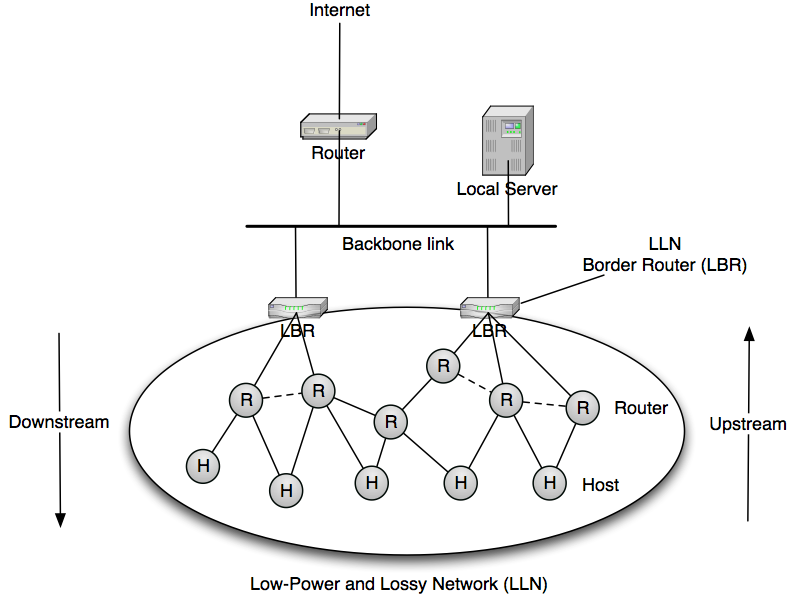
\includegraphics[width=.7\textwidth]{img/rpl.png}
	\caption{Schéma de l'architecture \ac{RPL}}
	\label{gw:fig:rpl_architecture}
\end{figure}

\ac{RPL} construit un graphe de routage entre les nœuds du \ac{LLN} et le routeur de bordure comme illustré sur la Figure~\ref{gw:fig:rpl_architecture}.
Le routage effectué par \ac{RPL} n'est valide qu'au sein du \ac{LLN} et s'arrête donc au \ac{LBR}.
Cette topologie est maintenue en utilisant aussi peu de messages de signalisation que possible.
Une fois construite, le protocole de routage maintient des routes montantes (\ac{MP2P} ou ``upstream'' en anglais) et descendantes (\ac{P2MP} ou ``downstream'' en anglais) et procède au routage des paquets IPv6.
La coordination du graphe de routage ainsi que la gestion du trafic doit être faite dans un lieu centralisé.
La passerelle peut assurer cette fonctionnalité de routeur de bordure en raison de ses ressources physiques et de sa position de racine.


% \begin{figure}[tb]
% 	\centering
% 	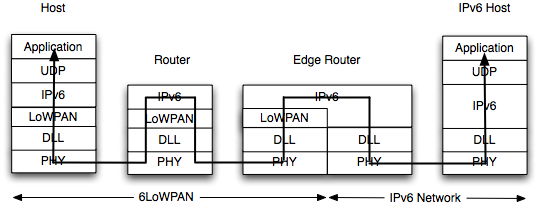
\includegraphics[width=.5\textwidth]{img/routing.png}
% 	\caption{Schéma de routage dans un \ac{LLN} à travers un routeur 6LoWPAN}
% 	\label{gw:fig:rpl_border}
% \end{figure}

Les nœuds routeurs disposant d'interfaces vers un autre lien IP sont appelés routeurs de bordure (\ac{LBR}), il peut y avoir plusieurs \ac{LBR} pour connecter un \ac{LLN} au reste d'un réseau afin d'assurer une redondance de lien de sorties souhaitable en cas de pannes.
Le rôle de \ac{LBR} est généralement accompli par la passerelle en raison des multiples interfaces de sorties dont elle dispose.

Les nœuds à l'intérieur du \ac{LLN} sont soit des routeurs soit des hôtes.
Les hôtes ne participent pas au routage et choisissent simplement un routeur par défaut, c'est par exemple le cas des nœuds fortement contraint qui ne peuvent assurer des tâches de routage pour le compte d'autres nœuds.
Les routeurs sont eux chargés de router les paquets en provenance d'hôte ou d'autres routeurs vers leur destination finale.

\subsubsection{Construction du routage}

Pour le routage montant (\ac{MP2P}), \ac{RPL} construit un \ac{DODAG} qui démarre à partir du \ac{LBR}.
Un rang est assigné à chaque nœud (routeur ou hôte) de tel sorte que le rang augmente à mesure que l'on s'éloigne du \ac{LBR}.
Router un paquet vers le \ac{LBR} consiste à choisir un voisin avec un rang aussi faible que possible.

Le routage descendant (\ac{P2MP}) peut être implémenté de manière stockée (``storing-mode'' en anglais) ou non stockée (``non storing-mode'' en anglais) à l'échelle du \ac{DODAG} entier.
Dans le cas où le routage descendant est non stocké, un routage à la source~\cite{rfc6554} est fait quand un paquet doit être routé vers un nœud spécifique dans le \ac{LLN}.
Le routeur de bordure indique la séquence de nœuds qu'il faut traverser pour que le paquet arrive à sa destination.
Le routeur de bordure apprend ce routage en collectant les \ac{DAO}s envoyés par chaque routeur vers le \ac{LBR} et qui indique parents et enfants du routeur en question.

Lorsque le routage descendant est stocké, des tables de routages intermédiaires sont utilisées pour qu'une route partielle soit construite à chaque nœud intermédiaire qui est capable de router le paquet dans son sous-réseau, jusqu'à ce que la destination finale soit atteinte.

\subsubsection{Maintenance du routage}

Les nœuds exécutant \ac{RPL} échangent des informations de signalisation pour mettre à jour le \ac{DODAG} et mettre à jour de manière proactive la topologie de routage.
Il existe plusieurs types de messages de signalisation, celui utilisé pour construire le \ac{DODAG} est un \ac{DIO}.
Tous les nœuds dans le réseau envoient régulièrement des \ac{DIO} afin d'indiquer leur rang à leur voisin.

\ac{RPL} peut détecter et réparer les boucles lorsque du trafic est envoyé dans le réseau et qu'une incohérence est détectée.
Par exemple, si un routeur reçoit un paquet ``descendant'' et qu'il doit l'envoyer à un nœud avec un rang plus faible ou un paquet ``montant'' et qu'il doit l'envoyer à un nœud avec un rang plus élevé alors une incohérence est détectée et une réparation locale est déclenchée.

La transmission des paquets est suspendue tant que le \ac{DODAG} n'est pas remis dans un état admissible ce qui peut occasionner des délais et des surcharges des mémoires tampons.

\paragraph{Limitation de trafic de routage (Trickle)}

\ac{RPL} utilise un mécanisme de timer adaptatif appelé  ``Trickle'' (goutte à goutte) afin de contrôler le débit d’émission des messages de signalisation (\ac{DIO}).
Trickle double l’intervalle séparant deux émissions successives de messages de contrôle à chaque fois que le réseau est cohérent, et ce jusqu’à une valeur maximale.
Ainsi le trafic \ac{RPL} diminue dans le réseau lorsqu'il est stable et que la topologie change peu.
Quand une incohérence est détectée, le timer est réinitialisé à sa valeur minimale et les mécanismes de réparation sont lancés.
Un des principaux avantages de l’utilisation du timer Trickle est qu’il ne nécessite pas de code complexe et il est assez facile à mettre en œuvre dans des nœuds disposant de ressources limitées.

\section{Interface applicative}
\label{gw:app_layer}

Un protocole applicatif a pour objectif de fournir un accès aux données et services applicatifs proposés.
Parmi les exemples les plus connus d'interface applicative, on peut citer l'accès à une page web, le transfert d'un fichier ou encore l'envoi de messages électroniques~\cite{pujolle2014reseaux}.
Cependant dans le cas des \ac{LLN}s, l'utilisation principale de cette interface applicative se borne à l'envoi d'instructions courtes et le relevé d'informations sur l'environnement immédiat des nœuds.
Ainsi il est nécessaire d'utiliser des protocoles aussi optimisés que possible pour ces usages.

\subsection{Contraintes de l'interface applicative d'un \ac{LLN}}

Les \ac{LLN}s doivent s'intégrer aussi facilement que possible aux services d'ores et déjà disponibles afin de faciliter leur adoption.
Une des clés de cette intégration et d'avoir une passerelle pouvant offrir une interface commune à de nombreux nœuds.
Enfin, il est impératif que cette intégration se fasse en consommant aussi peu de ressources que possible afin de garantir la durée de vie des nœuds et le bon fonctionnement du \ac{LLN}.

\subsubsection{Interface efficace avec les services web}

Les services web sont aujourd'hui la façon la plus utilisée pour interroger des serveurs de services~\cite{alonso2004web}.
Les ressources y sont désignées par une \ac{URI} qui assure l'adressage.
L'interaction avec cette \ac{URI} utilise d'une part le protocole \ac{HTTP}, et d'autre part une architecture \ac{REST} (Architecture client-serveur, absence d'états, etc.)~\cite{richardson2008restful}.

Afin de s'intégrer aussi facilement que possible à cette architecture, il est souhaitable pour les nœuds capteurs de disposer d'une sémantique proche et de disposer d'\ac{URI} pour désigner les ressources dont ils disposent.
Ainsi lorsqu'un développeur veut utiliser une source d'information en provenance d'un capteur, celle-ci doit être aussi simple à utiliser et proche de ses habitudes que possible.

\subsubsection{Disponibilités sur plusieurs plateformes}

L'objectif de la passerelle est de masquer les spécificités de chaque nœud capteur derrière un formalisme commun afin de simplifier la tâche des développeurs.
Ainsi, une couche applicative idéale doit pouvoir être implémentée sur un large ensemble de plateformes logicielles et matérielles.

\subsubsection{Contraintes en ressources}

Les nœuds capteurs offrant des services applicatifs disposent de peu de mémoire et de ressources de calculs.
Ainsi une couche applicative efficace doit avoir des entêtes aussi limités que possible, doit imposer aussi peu d'utilisation de mémoire que possible (par exemple pour conserver un état) et doit permettre de supporter des notifications afin d'éviter de payer le coût de requête typique des protocoles synchrones et très coûteux pour les \ac{LLN}s.

\subsection{État de l'art sur les protocoles applicatifs}

Il existe de nombreux protocoles applicatifs pouvant être appliqués aux \ac{LLN}s~\cite{karagiannis2015survey}.
L'objectif de ces couches applicatives consiste à faire un compromis entre jeu de fonctionnalités, interopérabilité et consommation énergétique.

\subsubsection{Couches spécifiques à une architecture matérielle}

Les piles protocolaires totalement intégrées dans un seul standard (Zigbee~\cite{zigbeeCritic} ou \ac{BLE}~\cite{bleCritic}) proposent leur propre couche applicative standardisée qui peut être prise en charge par la passerelle.

L'avantage de cette approche est qu'elle permet de disposer d'une couche applicative certifiée et d'un fonctionnement interopérable avec tous les appareils supportant la même norme.
Cependant ces couches protocolaires ne sont disponibles que sur leur matériel propre et sont donc peu interopérables avec des nœuds hétérogènes.

\subsubsection{\ac{MQTT}}

\ac{MQTT}~\cite{hunkeler2008mqtt} est un protocole standardisé par IBM reposant sur un mécanisme de publication-souscription (``publish-subscribe'' en anglais, ou ``pub-sub'' en abrégé) utilisé pour permettre à des abonnés (par exemple des services à valeur ajoutée) de s'abonner aux mises à jour envoyées par des nœuds de manière asynchrone.

L'avantage de ce protocole est d'avoir de nombreuses implémentations, un mode de fonctionnement particulièrement adapté aux notifications et un large support via de nombreuses bibliothèques logicielles~\cite{stanford2008mqtt}.

Cependant, ce protocole repose sur \ac{TCP} qui n'est pas véritablement adapté au contexte des \ac{LLN}s car les retransmissions qu'il induit consomment bande passante et énergie.
De plus, ce protocole n'offre pas d'interface directe vers les mécanismes de services web et leur paradigme \ac{REST} sans l'utilisation d'un service tiers avec maintien d'un état~\cite{collina2012introducing}.

\subsubsection{Application directe de \ac{HTTP}}

Utiliser \ac{HTTP} directement sur les nœuds capteurs permettrait d'avoir une pile applicative classique et directement compatible avec les services web usuels.
\ac{HTTP} est largement diffusé, disponible dans de nombreux langages nativement et dispose d'une sémantique puissante via l'utilisation de \ac{REST}.

Cependant, appliquer cette approche sur les \ac{LLN}s serait coûteux car l'utilisation de \ac{HTTP} implique celle de \ac{TCP} qui n'est pas adapté pour des nœuds très contraints en raison des retransmissions.
De plus, cette approche ne supporte pas pour le moment les notifications de type ``push'' car les services web fonctionnent de manière synchrone or des communications asynchrones sont très courantes dans le cas des \ac{LLN}s par exemple pour envoyer une notification quand une condition sur l'environnement se produit.

Ainsi il est nécessaire de chercher une synthèse proposant à la fois une intégration efficace avec des services web pour faciliter l'adoption des \ac{LLN}s comme source de données pour des services web tout en utilisant un protocole applicatif peu consommateur d'énergie et un support des notifications asynchrones.

\subsection{Présentation de \ac{CoAP}}

Le groupe de travail \ac{CoRE} de l'\ac{IETF} a défini le protocole \ac{CoAP}~\cite{rfc7252} pour fournir une interface applicative générique tout en ajoutant des fonctionnalités spécifiques aux contraintes des \ac{LLN}s comme des entêtes courts et faciles à disséquer, le support de notifications asynchrones, etc.

\ac{CoAP} est le plus souvent implémenté sur un protocole de transport orienté datagramme tel que \ac{UDP} afin d'avoir des entêtes courts qui nécessitent peu de bande passante.
Ainsi il implémente un mécanisme de transport unicast pour assurer une fiabilité sans utiliser un protocole dédié comme \ac{TCP} qui peut être plus complexe à implémenter pour les nœuds capteurs et consomme plus de ressources.

\ac{CoAP} utilise une architecture \ac{REST} reposant sur des verbes usuels comme \texttt{GET}, ou \texttt{PUT} permettant ainsi de disposer d'une sémantique riche directement dans le protocole sans nécessiter le maintien d'état en mémoire pour le capteur qui serait coûteux dans le cas de mémoire contrainte.

\subsubsection{Support de notifications asynchrones}

\ac{CoAP} supporte les notifications asynchrones afin de permettre à des nœuds capteurs d'envoyer des notifications sur un modèle ``push'' à un observateur.

En pratique, il n'y a le plus souvent qu'un seul observateur afin de limiter l'utilisation des ressources d'un nœud capteur qui n'a besoin de garder qu'une seule adresse en mémoire.
Dans cette architecture c'est le plus souvent un service qui va recueillir les notifications en provenance des nœuds capteurs et les distribuer vers les abonnés pertinents sans solliciter les nœuds capteurs.
Ce mode de fonctionnement peut être accompli par l'utilisation d'un proxy inversé (\ref{gw:reverse_proxy}).

\subsubsection{Traduction \ac{HTTP}/\ac{CoAP}}

L'un des objectifs de \ac{CoAP} est de permettre une traduction facile entre une \ac{URI} utilisée par un service web et celle qui est utilisée pour désigner la ressource d'un nœud capteur facilitant ainsi le travail des développeurs et l'intégration des \ac{LLN}s.

\ac{CoAP} n'est pas une compression naïve de \ac{HTTP} qui serait un standard complexe à implémenter et surdimensionné pour les nœuds capteurs.
La conversion entre \ac{HTTP} et \ac{CoAP} se fait sur les verbes employés (\texttt{GET}, \texttt{PUT}, etc.) et les \ac{URI} (paramètres et options compris).
La conversion est sans état et peut être faite efficacement par l'utilisation de proxy traducteurs situés entre les sources des requêtes \ac{HTTP} et les nœuds capteurs.

De plus, \ac{CoAP} supporte le traitement complet d'une \ac{URI} afin de profiter des options qu'elle contient pour répondre plus précisément à une requête (par exemple recevoir une notification si la température dépasse un seuil.)

\subsection{Traduction, proxy inversé et cache}
\label{gw:rpc}

La passerelle peut offrir une médiation applicative entre les \ac{LLN}s et les fournisseurs de services à valeur ajoutée.
Cette médiation peut être approfondie par la passerelle afin d'offrir des fonctionnalités supplémentaires ayant pour objectif d'améliorer la rapidité du traitement d'une requête et limiter la consommation énergétique des nœuds du \ac{LLN}.

\subsubsection{Traduction}
\label{gw:traduction}

Les nœuds d'un \ac{LLN} utilisent des protocoles applicatifs hétérogènes et les fournisseurs de services veulent éviter d'implémenter un support pour un grand nombre de protocoles qui serait trop coûteux.
La passerelle connaît les spécificités de chaque nœud et peut offrir des traductions de protocoles depuis des protocoles usuellement utilisés dans les services web tel qu'\ac{HTTP} vers les protocoles utilisés par les nœuds capteurs du \ac{LLN}.
Ainsi les tâches de traduction se font au plus près des nœuds capteurs et permet de simplifier le traitement des données dans des architectures orientées service.

\subsubsection{Proxy inversé}
\label{gw:reverse_proxy}

La fonctionnalité de traduction n'est pas suffisante pour fournir un service efficace et sécurisé.
En effet, les nœuds capteurs étant contraints ils ne peuvent recevoir qu'une quantité limitée de trafic.
De plus, s'ils sont accessibles depuis un réseau public, il est nécessaire de contrôler finement le trafic reçu afin d'éviter par exemple des attaques par déni de service ou de sommeil~\cite{wessels2001web,raymond2008denial}.

Un proxy inversé (``reverse proxy'' en anglais)~\cite{reese2008nginx} est un serveur qui se pose entre des requêtes provenant de l'extérieur et des services à protéger comme représenté sur la Figure~\ref{gw:fig:rpc}.
Le proxy inversé intercepte l'ensemble des requêtes à destination des nœuds et peut les modifier, les faire passer ou renvoyer des codes d'erreurs.

Le proxy inversé se pose en intermédiaire permettant un gain en termes de fonctionnalité  appréciable, car un administrateur peut configurer le proxy inversé pour gérer le trafic applicatif reçu par les nœuds au lieu de le configurer individuellement sur chaque nœud.
Ainsi l'administrateur du \ac{LLN} peut limiter arbitrairement les requêtes transmises aux nœuds pour limiter l'énergie qu'ils consommeraient pour y répondre.

De plus, dans le cas de notifications asynchrones, avoir un proxy inversé qui centralise les notifications est pertinent, car les nœuds capteurs ne doivent envoyer de notifications que vers une seule destination.
Lorsque la notification est arrivée sur le proxy inversé il se charge de distribuer cette notification vers les abonnés pertinents.
Ainsi la gestion d'un grand nombre d'abonnés est déportée des nœuds capteurs vers le proxy inversé et une économie d'énergie est ainsi réalisée.

\subsubsection{Cache}
\label{gw:cache}

Un cache stocke du contenu afin de l'avoir à disposition sans le redemander au reste du réseau.
Une économie de bande passante et de délai est donc réalisée à chaque fois qu'une requête est traitée par l'utilisation d'un cache au lieu d'être envoyée aux nœuds du \ac{LLN}~\cite{wessels2001web}.
À ce titre, le rapport entre le nombre de requêtes traitées par le cache sur le nombre de requêtes total (``hit rate'' en anglais)  est une métrique importante pour mesurer son efficacité.
Il est nécessaire d'avoir une politique de mise en cache, car la quantité de mémoire du cache est limitée, de plus, une information peut devenir obsolète si elle reste en cache trop longtemps.

L'utilisation d'un cache est étudiée dans les \ac{LLN}s~\cite{colitti2011rest} et notamment avec \ac{CoAP} car elle permet de faire des économies de bande passante et d'accélérer le traitement d'une requête~\cite{rfc7641}.

\subsection*{Conclusion intermédiaire}

Comme vu dans cette section, \ac{CoAP} permet d'offrir une sémantique et un jeu de fonctionnalités riches comme le support de messages asynchrones et la traduction sans état avec \ac{HTTP} tout en consommant aussi peu d'énergie que possible.

Cette intégration des notifications asynchrones est d'autant plus pertinente que les versions futures de \ac{HTTP}2 en cours de déploiement supporteront les notifications asynchrones (``push notifications'' en anglais).
Ainsi, des traductions sémantiquement complètes pourront être mises en œuvre entre \ac{CoAP} et \ac{HTTP}2.
Ces aspects sont activement étudiés aujourd'hui et accentue la nécessité d'avoir des traductions aussi efficaces que possible autour du paradigme \ac{REST} entre les nœuds et les fournisseurs de services à valeur ajoutée ce que \ac{CoAP} fournit.

\begin{figure}[ht]
  \centering
  \begin{tikzpicture}

  % définition des styles
  \tikzstyle{visible}=[draw, fill=blue!50]
  \tikzstyle{hidden}=[ draw, fill=gray!20]
  \tikzstyle{router}=[circle, draw, fill=orange!50,text=black]
  \tikzstyle{child}=[circle, draw, fill=yellow!50,text=black]
  \tikzstyle{root}=[circle, draw, fill=red!50,text=black]

  % les nœuds
  \node[draw] (gw) {Reverse Proxy};

  \node[draw, above= of gw] (cache) {Cache};


  % Réseau contraint
  \node[root] (1) at (-4, 0) {};
  \node[router] (2) at (-5, 1) {};
  \node[child] (3) at (-5, -1) {};
  \node[child] (4) at (-6, 2) {};
  \node[child] (5) at (-6, 0) {};

  % \node[cloud, cloud puffs = 10, minimum width = 4cm, draw, fill = gray!10] (cloud) at (5,0) {Réseau local};
  \node[draw] (cloud) at (5,0) {Réseau local};

 \node [fit=(1) (2) (3) (4) (5), rounded corners, draw=black!50] (lln) {};
 \node [below=.3 cm of lln] {LLN};

\path

  % Réseau contraint
  (gw.west) edge[<-, cyan, thick, bend left=20] node [below] {CoAP 2.05} (1) 
  (gw.west) edge[->, olive, thick, bend right=20] node [above] {CoAP GET} (1) 
  (1) edge[<->] (2)
  (1) edge[<->] (3)
  (2) edge[<->] (4)
  (2) edge[<->] (5)

  (cache) edge[->, very thick, cyan, bend right=20] (gw)
  (cache) edge[<-, very thick, cyan, bend left=20] (gw)

  % Réseau conventionnel
  (gw.east) edge[<-, olive, very thick, bend left=20] node [above] {GET / HTTP/1.1} (cloud.west)
  (gw.east) edge[->, cyan, very thick, bend right=20] node [below] {HTTP/1.1 200 OK} (cloud.west)
  ;

  \end{tikzpicture}
  
  \caption{Architecture d'un \ac{RPC}}
  
  \label{gw:fig:rpc}
\end{figure}

\ac{CoAP} permet de plus l'utilisation de fonctionnalités au niveau de la passerelle afin d'accélérer le traitement des requêtes et économiser de la bande passante.
Ces fonctionnalités de traductions entre \ac{HTTP} et \ac{CoAP}, de proxy inversé et de cache sont dénommées \acl{RPC} et sont résumées sur la Figure~\ref{gw:fig:rpc}.
Cette figure illustre l'exemple de l'envoi d'une requête \ac{HTTP} qui est traduite en CoAP avant d'être envoyée dans le \ac{LLN}.
Une fois la réponse \ac{CoAP} obtenue, elle est retraduite en réponse \ac{HTTP} puis mise en cache afin d'être réutilisée ultérieurement enfin la réponse \ac{HTTP} est fournie au client.

En raison de sa pertinence, \ac{CoAP} sera le protocole applicatif utilisé dans le reste de cette thèse.

\section{Supervision}
\label{gw:supervision}

La supervision désigne la surveillance continue d'un système afin de s'assurer que son fonctionnement et ses performances sont ceux attendus~\cite{ligus2012effective}.

Cette surveillance est nécessaire pour s'assurer par exemple qu'un système d'acquisition est toujours valide ou bien que ses réserves d'énergies sont suffisantes pour tenir pendant une durée donnée.
Un système de supervision peut agir en envoyant une alerte à un humain ou un autre système pour l'informer qu'un \ac{LLN} rencontre des problèmes et qu'une intervention est peut-être à prévoir.
Son objectif est alors de permettre à un administrateur d'identifier aussi rapidement que possible quel est le problème et ses causes.

Dans le cas des \ac{LLN}s, les métriques recueillies peuvent être relatives à un nœud donné par sa consommation énergétique, l'état du médium, le nombre de retransmissions, la charge moyenne, etc.
Ou bien relatives à l'ensemble du \ac{LLN}s avec les nœuds les plus sollicités, les nœuds ayant des ressources énergétiques en dessous d'un certain seuil, la latence globale ou les erreurs applicatives, etc.

Toutes ces informations permettent de prendre des décisions motivées et justifiées sur la maintenance du réseau afin de garantir son fonctionnement.

\subsection{Fonctionnalités recherchées}

La supervision couvre plusieurs aspects fonctionnels et administratifs du fonctionnement d'un système.
Sa mise en place repose sur plusieurs objectifs fonctionnels et techniques.

\subsubsection{Suivi des équipements}

Un premier objectif de la supervision dans un \ac{LLN} consiste à connaître l'ensemble des équipements déployés, leurs fonctionnalités, depuis quand ils sont en fonctionnement.
Cette fonctionnalité d'inventaire peut être complexe à mettre en place dans le cas où les équipements changent dynamiquement et sont fortement hétérogènes.

Ce suivi des équipements est utile pour diagnostiquer des problèmes temporels pouvant survenir lors de l'ajout de matériel.
Par exemple, l'ajout d'un trop grand nombre de nœuds physiques avec une certaine configuration peut causer une perte de performance selon certaines métriques, etc.

\subsubsection{Suivi de la disponibilité}

La supervision permet d'obtenir une distinction entre un suivi dans le temps de la disponibilité matérielle et fonctionnelle d'un système qui est nécessaire pour avoir un suivi de supervision efficace.
Dans le cas d'un \ac{LLN} appliqué à un scénario de bâtiment intelligent, une supervision de disponibilité matérielle permet de savoir, par exemple, si un nœud physique donné est disponible.
Une supervision de disponibilité fonctionnelle, quant à elle, permet de savoir s'il est possible de mesurer la température sur un étage donné d'un bâtiment.

Cette distinction est essentielle afin d'avoir des alertes de supervision pertinentes et de ne solliciter des interventions humaines coûteuses uniquement pour les problèmes  critiques.

\subsubsection{Prévision}

Un autre volet important de la supervision consiste à analyser les tendances de fond d'un système afin de prévoir son fonctionnement.
Prévoir l'évolution d'une métrique permet d'éviter des accidents d'exploitations ou d'autres pannes pouvant survenir lors de l'évolution d'un \ac{LLN}.
En outre, cette prévision permet de séparer les problèmes et les alertes en fonction de leur urgence et de permettre des interventions humaines plus flexibles dans le temps.

\subsubsection{Construction de tableau de bord}

Les tableaux de bord (en anglais ``dashboards'') permettent d’agréger et de filtrer les métriques nombreuses et hétérogènes d'un système afin de ne présenter à un administrateur humain que les métriques les plus pertinentes.
Ainsi l'administrateur dispose d'une interface qui peut être une visualisation graphique comme une ``WeatherMap''~\cite{haiyan2008application} capable de représenter visuellement l'état de tous les équipements déployés afin de prendre rapidement une décision à propos d'une situation ou bien demander l'intervention d'un technicien.

\subsection{Problématiques de la supervision pour les \ac{LLN}s}

Les remontées périodiques d'informations permettent d'obtenir un état sur chaque nœud physique afin de pouvoir l'interpréter. 
Cependant, ce coût de supervision impacte les réserves d'énergie des nœuds et devrait être réduit autant que possible tout en permettant un niveau minimum de fiabilité sur le déploiement.
Ainsi les problématiques de déploiements des \ac{LLN}s doivent réaliser un compromis entre consommation des ressources et informations gagnées.

De plus, la supervision dans les \ac{LLN}s rencontre d'autres difficultés techniques pour sa mise en place.

\subsubsection{Contraintes physiques et logicielles}

Les techniques de supervision usuelles reposent le plus souvent sur l'hypothèse qu'un nœud peut toujours répondre aux requêtes de supervision~\cite{ward2014observing}.
Cette hypothèse n'est en général pas validée dans le cas des \ac{LLN}s.

D'une part, les nœuds d'un \ac{LLN} ont des ressources limitées: répondre à des requêtes de supervision trop fréquentes peut causer un coût important aussi bien sur leur énergie que sur la bande passante disponible et ainsi compromettre leurs objectifs.

D'autre part, il peut être coûteux d'implémenter une solution de supervision pour l'ensemble des nœuds, car les ressources en mémoire et en architecture matérielle ne le permettent peut-être pas (pas de support pour les nombres flottants, pas assez d'espace mémoire, etc.).
De plus, dans le cas où l'administrateur n'a pas la main sur le code s'exécutant sur un nœud, déployer un agent spécifique devient alors inenvisageable.

\subsubsection{Grande hétérogénéité}

Un autre problème pour la supervision des \ac{LLN}s provient de la grande hétérogénéité des nœuds physiques et de l'interprétation des métriques.
Une métrique au-delà d'un certain seuil peut être acceptable pour certains nœuds, mais pas pour d'autres (par exemple le niveau de batterie, l'espace mémoire flash disponible).
Ainsi la définition des alertes et des seuils est complexe et très dépendante d'un contexte donné.

\section{Conclusion}
\label{gw:conclusion}

\begin{figure}[ht]
  \centering
  \begin{tikzpicture}
    \tikzstyle{block} =[draw, fill=white,rectangle, minimum width={width("\ieee{}")+2pt}, minimum height=.75cm, font=\small]

      \node [fill=yellow!30, draw=black!50] (llnNode) {
        \begin{tikzpicture}

          \node[block] (ieee802154) {\ieee{}};
          \node[block, above=0 of ieee802154] (lowpan) {6LoWPAN};
          \node[block, above=0 of lowpan](udp){UDP};
          \node[block, above=0 of udp](coap){CoAP};

        \end{tikzpicture}
      };
      \node [above=0.3cm of llnNode] {Hôte};

      \node [fill=orange!30, draw=black!50, right=.3cm of llnNode] (llnRouter) {
        \begin{tikzpicture}

          \node[block] (ieee802154) {\ieee{}};
          \node[block, above=0 of ieee802154] (lowpan) {6LoWPAN};
          \node[block, above=0 of lowpan](udp){UDP};
          \node[block, above=0 of udp](coap){CoAP};

        \end{tikzpicture}
      };
      \node [above=0.3cm of llnRouter] {Hôte et Routeur};

      \node [fill=red!30, draw=black!50, right=.3cm of llnRouter] (llnGateway) {
        \begin{tikzpicture}

          \node[block] (ieee802154) {\ieee{}};
          \node[block, above=0 of ieee802154] (lowpan) {6LoWPAN};
          \node[block, above=0 of lowpan](udp){UDP};
          \node[block, above=0 of udp](coap){CoAP};

          \node[block,right=of ieee802154] (ethernet) {Ethernet/Wifi};
          \node[block,above=0 of ethernet](ip){IPv4/IPv6};
          \node[block,above=0 of ip](tcp){TCP};
          \node[block,above=0 of tcp](http){HTTP};

          \path
          (lowpan) edge[>=latex, <->, ultra thick] (ip)
          (coap) edge[>=latex, <->, ultra thick]  (http)
          ;


        \end{tikzpicture}
      };
      \node [above=0.3cm of llnGateway] {Passerelle \& Reverse proxy};

      \node [fill=green!30, draw=black!50, right=.3cm of llnGateway] (server) {
        \begin{tikzpicture}

            \node[block] (ethernet) {Ethernet/Wifi};
            \node[block,above=0 of ethernet](ip){IPv4/IPv6};
            \node[block,above=0 of ip](tcp){TCP};
            \node[block,above=0 of tcp](http){HTTP};

        \end{tikzpicture}
      };
      \node [above=0.3cm of server] {Hôte};

      \path
      ([yshift=-5pt]llnNode.south west) edge[>=latex, <->, ultra thick] node[below] {6LoWPAN} ([yshift=-5pt]llnGateway.south)
      ([yshift=-5pt]llnGateway.south) edge[>=latex, <->, ultra thick] node[below] {IP} ([yshift=-5pt]server.south east)
      ;

  \end{tikzpicture}

  \caption{Schéma de l'acheminement des requêtes dans un \ac{LLN}}

  \label{gw:fig:stacks}
\end{figure}

L'échange de messages sur un réseau \ac{LLN} repose sur un ensemble de couches (au même titre qu'un réseau classique) optimisées afin de minimiser les consommations d'énergie et de bande passante.
Ces économies sont faites au niveau des couches basses (\ref{gw:low_layers}), de la compression des en-têtes (\ref{gw:6lowpan}), des stratégies de routages (\ref{gw:routing}) et de la mise en cache de messages applicatifs (\ref{gw:app_layer}).
La Figure~\ref{gw:fig:stacks} propose un récapitulatif des protocoles mis en jeu lors des déploiements typiques qui ont été faits pendant cette thèse ainsi que les traductions faites au niveau de la passerelle.

Comme vu dans la section~\ref{gw:supervision}, la supervision est un aspect critique du déploiement d'un \ac{LLN} afin de s'assurer qu'il fonctionne de manière normalement.
Les approches actuelles reposent essentiellement sur des envois systématiques d'information de supervision qui induisent une charge croissante à mesure que le \ac{LLN} grandit, notamment si la fréquence d'émission de ces messages est élevée.
Le chapitre~\ref{supervision} montre comment fournir un mécanisme de mesure implicite de la consommation énergétique d'un nœud en inférant l'utilisation de sa radio à partir du trafic réseau rentrant et sortant du \ac{LLN} et de la topologie de routage.

Comme vu dans la sous-section~\ref{gw:rpc}, les \acl{RPC} permettent de réduire le trafic applicatif reçu par les nœuds capteurs en répondant à la place des nœuds du \ac{LLN}.
Pour cela, le \acl{RPC} garde en mémoire pour un certain temps de validité les réponses des requêtes visant les nœuds.
Les approches actuelles ne modulent pas ce temps de validité en fonction des objectifs de durée de vie du réseau.
Le chapitre~\ref{cache} montre comment adapter les temps de validité utilisés par le \ac{RPC} afin d'adapter la quantité de trafic admise dans le \ac{LLN}.
Ce mécanisme utilise la topologie fournie par le protocole de routage du \ac{LLN} et une mesure du trafic entrant pour fournir des temps de validité optimaux pour un objectif de durée de vie donné.
